% =============================================================================
% ch02_bio_basis.tex — Chapter 2: Biological Basis | Biomimetic Navigator
% =============================================================================

\selectlanguage{hebrew}
\section{הבסיס הביולוגי: אקולוקציה ועיבוד שמע של עטלפים}
\label{sec:bio_basis}

\subsection{מבוא לאקולוקציה ביומימטית}
עטלפים ממשפחת ה-\en{Rhinolophidae} (עטלפי-פרסה) פיתחו את אחת ממערכות הניווט המתוחכמות ביותר בטבע. בניגוד לרוב היונקים המסתמכים על ראייה, העטלפים משתמשים באנרגיה אקוסטית כדי למפות את סביבתם בתלת-ממד, לזהות טרף ולנווט במנהרות ויערות סבוכים בחשיכה מוחלטת. \cite{GriffinBatEcholocation}

\subsection{מבנה האות האקוסטי: פולסי CF/FM}
אות האקולוקציה של עטלפי הפרסה מורכב ממבנה תלת-שלבי: \en{iFM-CF-tFM}.
\begin{enumerate}
    \item \textbf{שלב ה-\en{CF} (Constant Frequency):} רכיב זה מהווה את עיקר הפולס (10–50 \en{ms}). הוא משמש לזיהוי מהירות יחסית באמצעות אפקט דופלר (\en{Doppler Shift}).
    \item \textbf{שלבי ה-\en{FM} (Frequency Modulated):} פולסי ה-\en{FM} בתחילת ובסוף האות משמשים למדידת טווח (\en{ranging}) מדויקת.
\end{enumerate}

התדר המרכזי (\en{CF}) משתנה בין המינים, כפי שמוצג בטבלה \ref{tab:bat_species}:

\begin{table}[H]
\centering
\begin{tabular}{lccc}
\toprule
מין העטלף & תדר \en{CF} [\en{kHz}] & משך פולס [\en{ms}] & רזולוציית טווח [\en{mm}] \\
\midrule
\textit{R. ferrumequinum} & 83 & 40 & 2.1 \\
\textit{R. hipposideros} & 110 & 30 & 1.8 \\
\textit{R. mehelyi} & 106 & 35 & 1.9 \\
\bottomrule
\end{tabular}
\caption{מאפייני פולס האקולוקציה במיני עטלפים שונים.}
\label{tab:bat_species}
\end{table}

\subsection{עיבוד אקוסטי ב-\en{Cochleagram}}
החזר התיק (\en{echo}) מעובד בשבלול האוזן (\en{cochlea}) של העטלף, הפועל כמערך של מסנני תדר (\en{filter bank}). ייצוג זה, המכונה \en{Cochleagram}, מאפשר לעטלף להפריד בין רעשי רקע (\en{clutter}) לבין מטרות נעות. \cite{MossEcholocation}

\begin{figure}[H]
    \centering
    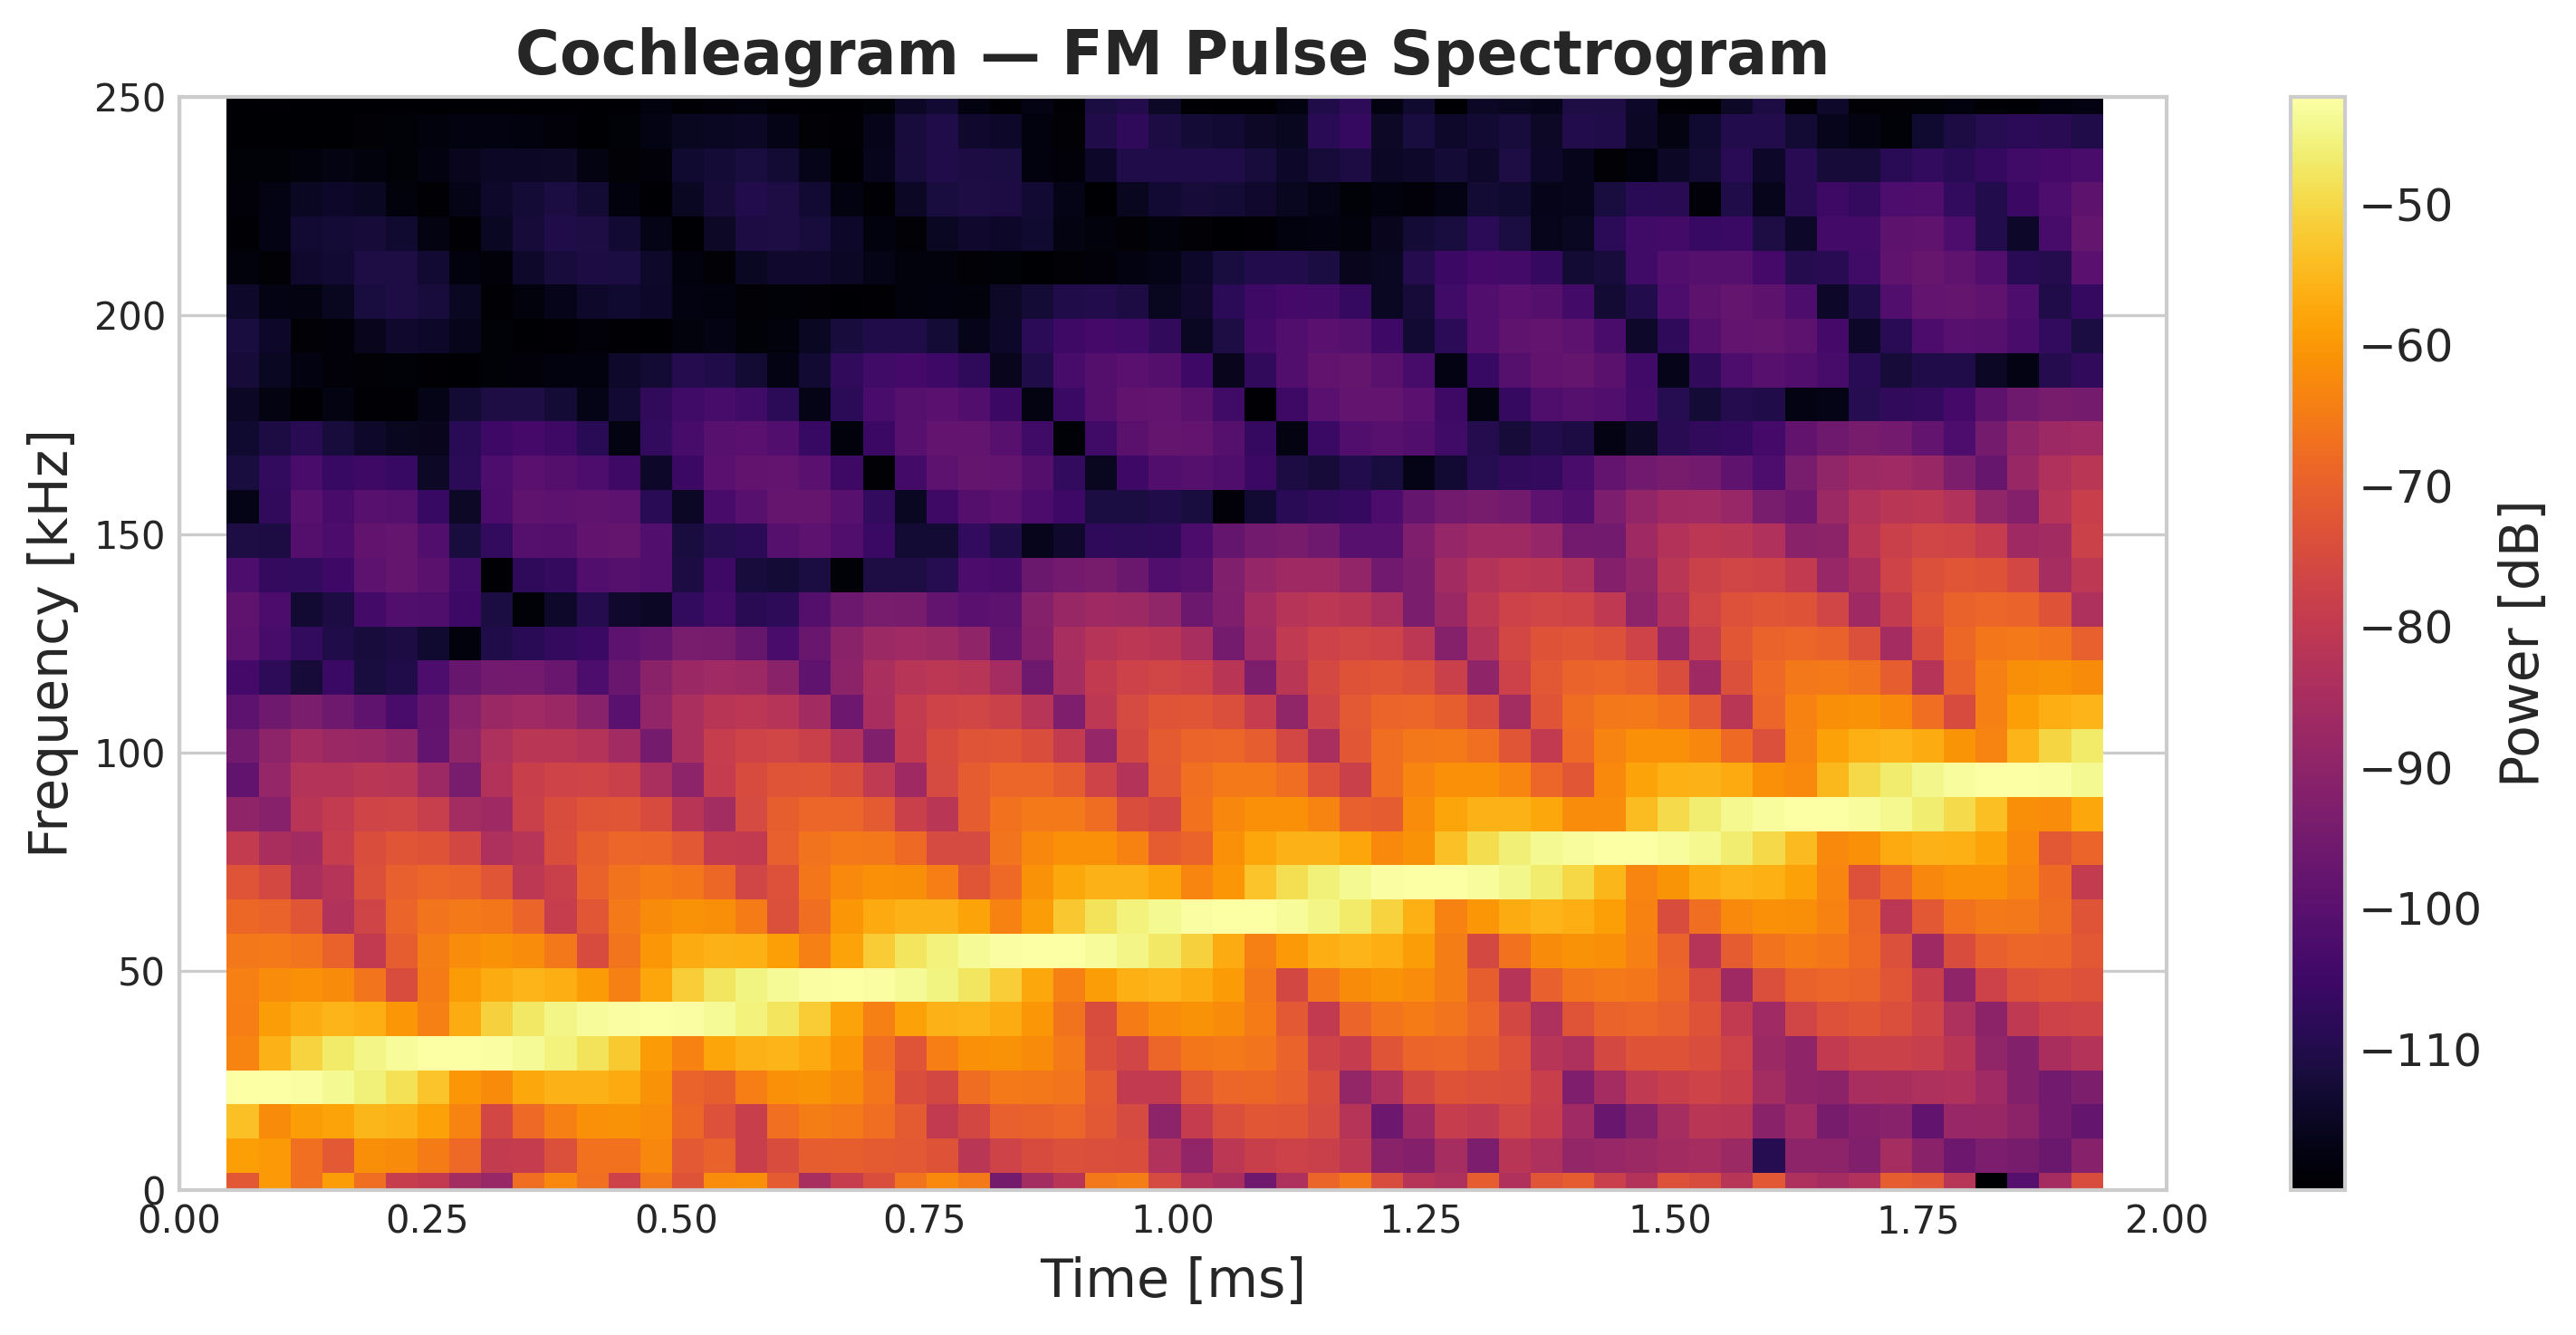
\includegraphics[width=0.8\columnwidth]{figures/fig_cochleagram.png}
    \caption{ייצוג \en{Cochleagram} של פולס \en{FM} סינתטי. ניתן לראות את השינוי הליניארי בתדר לאורך הזמן.}
    \label{fig:cochleagram}
\end{figure}

\subsection{פיצוי דופלר ומרחב השמע (\en{Acoustic Fovea})}
עטלפים אלו מפגינים יכולת מדהימה של פיצוי דופלר (\en{Doppler Shift Compensation}). הם משנים את תדר השידור שלהם כך שההחזר יתקבל תמיד בטווח התדרים שבו האוזן שלהם היא הרגישה ביותר — ה-\en{Acoustic Fovea}. \cite{Simmons1979BatSonar}
נוסחת היסט דופלר עבור מהירות $v$ ומהירות קול $c$ היא:
\begin{equation}
    f_r = f_s \left( \frac{c + v}{c - v} \right)
    \label{eq:doppler}
\end{equation}
יכולת זו קריטית לניווט של רחפנים במהירויות גבוהות, כפי שנתאר בפרק \ref{sec:algorithm}.
